In this section, we describe the instantiation of \name on
Cassandra~\cite{Cassandra}, a popular, industrial-strength, column-oriented,
distributed database. Cassandra offers eventual consistency with a
last-write-wins conflict resolution policy. Cassandra also offers complex data
types such as \texttt{list}, \texttt{set} and \texttt{map} with baked-in conflict resolution policies. Given the
richness of replicated data types, the available complex data types are quite
limiting. Cassandra also offers lightweight transactions (distributed
compare-and-update) implemented using the Paxos consensus
protocol~\cite{lamport2001paxos}. Lightweight transactions are limited to operate
on only one object. \name does not use lightweight transactions since their cost is prohibitively high due to consensus. As
mentioned previously \name only requires sticky availability, and so uses a
replica-local lock for ensuring mutual exclusion when multiple sessions try to
update the public branch on a replica concurrently.

By instantiating \name on Cassandra, we offload the concerns of replication,
fault tolerance, availability and convergence to the backing store. On top of
Cassandra, \name uses Irmin~\cite{Irmin}, an OCaml library for persistent
stores with built-in branching, merging and reverting facilities. Irmin can be
configured to use different storage backends, and in our case, the storage is
Cassandra. Importantly, Cassandra being a distributed database serves the
purpose of the networking layer in addition to persistent storage. While Irmin permits
arbitrary branching and merging, \name is a specific workflow on top of Irmin
which retains high availability.

\subsection{Irmin data model}

\begin{wrapfigure}{r}{0.5\textwidth}
	\vspace{-1.6cm}
	\centering
	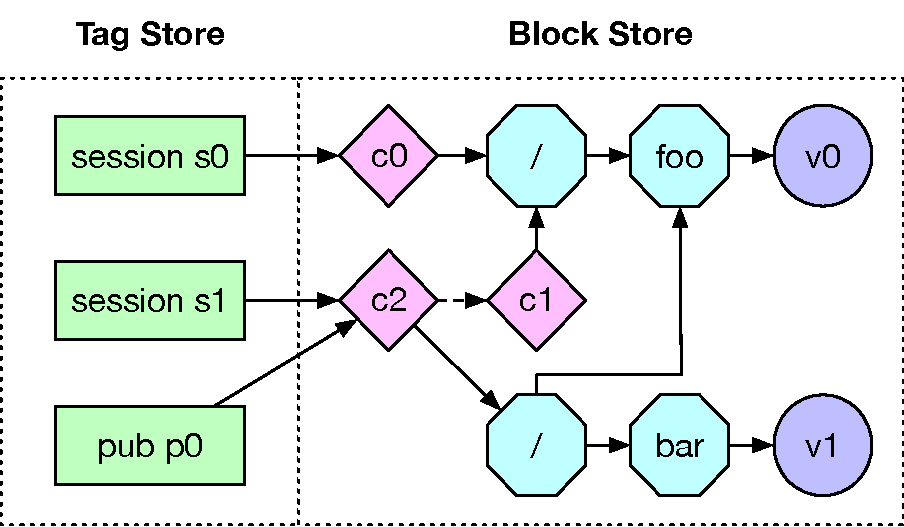
\includegraphics[scale=0.4]{figures/irmin_store}
	\caption{A sample Irmin store. The rectangles are tags, diamonds are commit
	objects, octagons are tree object, and circles are blob objects.}
	\vspace{-0.8cm}
	\label{fig:irmin_store}
\end{wrapfigure}
The expressivity of Irmin imposes significant burden on the underlying storage.
For efficiently storing different versions of the state as the store evolves,
Irmin uses the Git object model. Figure~\ref{fig:irmin_store} shows a snapshot
of the state of the Irmin store. There are two kinds of stores: a mutable tag
store and an immutable, content-addressed block store. The tag store records
the branches and the commit that corresponds to this branch. In this example,
we have three branches, |session s0|, |session s1| and |pub p0|.

The block store is content-addressed and has three different kinds of objects:
commits, tree and blobs. A commit object represents a commit, and it may have
several parent commits and a single reference to a tree node. For example, the
commit |c2|'s parent is |c1|, and |c0| and |c1| do not have any parent commits.
The tree object corresponds to directory entries in a filesystem, and
recursively refer to other tree objects or a blob object. Unlike Git, Irmin
allows blob objects to be arbitrary values, not just files. The blob objects
may refer to other blob objects. In the session |s1|, reading the keys
|["foo"]| and |["bar"]| would yield |Some v0| and |Some v1|, respectively.

Observe that all the commits share the tree object |foo| and its descendents,
thanks to the block store being content addressed. Content addressibility of
the block store means that as the store evolves, the contents of the store are
shared between multiple commits, if possible. On the other hand, updating a
value in a deep hierarchy of tree objects would necessitate allocating a new
spine in order to maintain both the old and the new versions. Thus, each write
in \name will turn into several writes to the underlying storage.

\subsection{Cassandra instantiation}

For instantiating \name on Cassandra, we use two tables, one for the tag store
and another for the block store. For the tag store, the key is a |string| (tag)
and the value is a |blob| (hash of the commit node). For the block store, the
key is a |blob| (hash of the content), and the value is a |blob| (content).
Irmin handles the logic necessary to serialize and deserialize the various Git
objects into binary |blob|s and back.

Cassandra replicates the writes to the tag and block tables asynchronously
amongst the replicas. Each replica periodically merges the public branches of
other replicas into its public branch to fetch remote updates. Due to eventual
consistency of Cassandra, it may be the case that not all the objects from a
remote replica are available locally. For example, the merge function may find
a new commit from a remote replica, but the tree object referenced by a commit
object may not available locally. In this situation, \name simply skips merging
this branch in this round. Cassandra ensures that eventually the remote tree
object will arrive at this replica and will be merged in a subsequent remote
refresh operation. Thus, fetching remote updates is a non-blocking operation.

In Irmin, the tag store is update with a compare-and-swap to ensure that
concurrent updates to the same tag should be disallowed. Naively implementing
this in Cassandra would necessitate the use of lightweight transactions and
suffer prohibitive costs. By restricting the \name programming model
(Section~\ref{sec:model}) such that entries in the tag store (in particular,
the tag corresponding to the public branch of the replica) is only updated on
that replica, we remove the necessity for lightweight transactions. Thus, we
do not depend on any special features of Cassandra to realise the \name model,
and \name can be instantiated on any eventually consistent key-value store.

\subsection{Recursive merges}
\label{sec:rec_merge}

A particular challenge in making \name scalable is the problem of recursive
merges. Consider a simple mergeable counter MRDT, whose implementation is:
\begin{lstlisting}
let merge lca v1 v2 =
let old = match lca with None -> 0 | Some v -> v in
v1 + v2 - old
\end{lstlisting}

\begin{wrapfigure}{r}{0.45\textwidth}
	\centering
	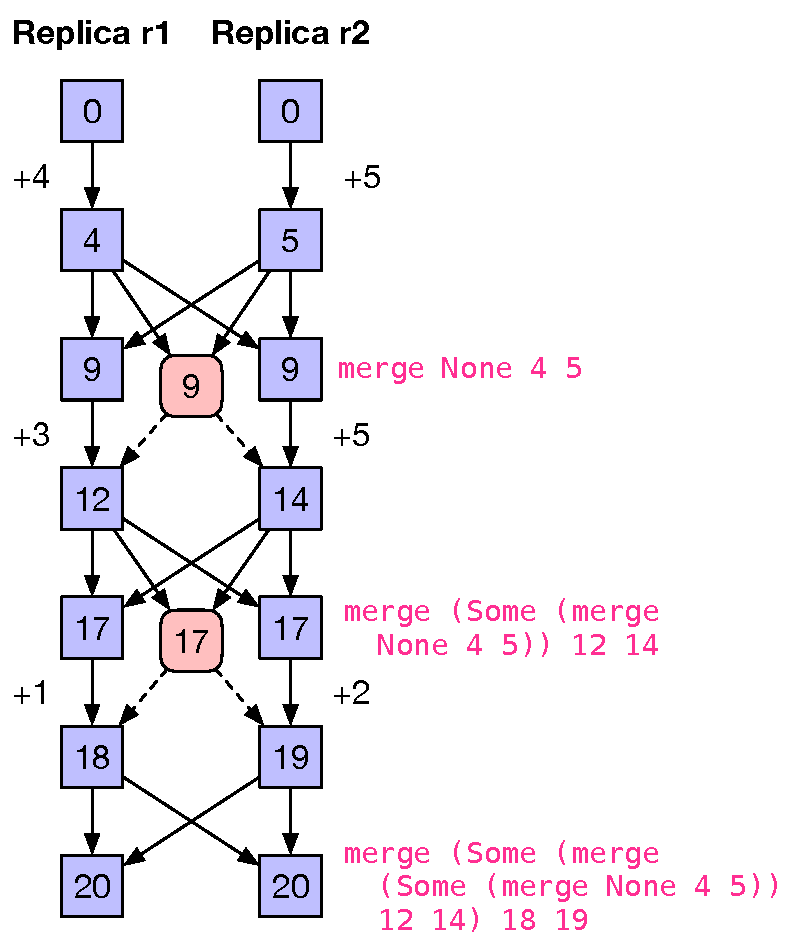
\includegraphics[scale=0.45]{figures/recursive}
	\caption{Recursive merge. Rounded rectangles are the results of recursive
		merges.}
	\label{fig:recursive}
	\vspace{-0.9cm}
\end{wrapfigure}
Consider the execution history presented in Figure~\ref{fig:recursive} which
shows the evolution of a single counter. The history only shows the interaction
between two replicas, and does not show any sessions. Each node in the history
is a commit. Since we want to focus on a single counter, for simplicity, we
ignore the tree nodes and the node labels show the counter value.

Initially the counters are |0|, and each replica concurrently increments the
counter by |4| and |5|. When the replicas perform remote refreshes, they invoke
|merge None 4 5| to resolve the conflict updates yielding |9|. The LCA is
|None| since there is no common ancestor.

Subsequently, the replicas increment the counters by |3| and |5|. Now, consider
that the replicas merge each other's branches. When merging |12| and |14|,
there are two equally valid LCAs |4| and |5|. Picking either one of them leads
to incorrect result. At this point, Irmin merges the two LCAs             using
|merge None 4 5| to yield |9|, which is used as the LCA for merging |12| and
|14|. This yields the value |17|. The result of merging the LCAs is represented
as a rounded rectangle. Importantly, the result of the recursive merge |9| is
not a parent commit of |12| and |14| (distinguished by the use of dotted
arrows). This is because the commit nodes are stored in the content-addressed
store, and adding a new parent to the commit node would create a distinct node,
whose hash is different from the original node. Any other nodes that referenced
the original commit node will continue to reference the old node. As a result,
the recursive merges will need to be performed again for subsequent requests!

Consider that the replicas further evolve by incrementing |1| and |2|, yielding
|18| and |19|. When these commits are merged on remote refresh, there are two
LCAs |12| and |14|, which need to be merged. This in turn has two LCAs |4| and
|5|, which need to be merged. Thus, every subsequent recursive merge, which is
very likely since the replicas merge each other's branches, requires repeating
all the previous recursive merges. This does not scale.

We solve this problem by having a separate table in Cassandra that acts as a
cache, recording the result of LCA merges. Whenever \name encounters a
recursive merge, the cache is first consulted before performing the merge. In
this example, when |18| and |19| are being merged, \name first checks whether
the two LCAs |12| and |14| are in the cache. They would not be. This triggers a
recursive merge of LCAs |4| and |5|, whose result is in the cache, and is
reused. The cache is also updated with an entry that records that the merge of
the LCAs |12| and |14| is the commit corresponding to |17|.

\subsection{Garbage collection}
\label{sec:gc}

While traditional database systems only store the most recent version of the
data, \name necessitates that previous versions of the data must also be kept
around for three-way merges. While persistence of prior
versions~\cite{Driscoll86,farinier15} is a useful property for audit and tamper
evidence, the \name API presented here does not provide a way to access earlier
versions. The question then is: when can those prior versions be garbage
collected?

We have not yet implemented the garbage collector for \name on Cassandra, but we
sketch the design here. Git is equipped with a garbage collector (GC) that
considers that any object in the block store that is reachable from the tag
store is alive. Unreachable objects are be deleted. Our aim is to assist the
Git-like GC by pruning the history graph of nodes which will no longer be used.
The key idea is that if a commit node will not be used for LCA computation,
then that commit node may be deleted. Deleting commit nodes will leave dangling
references from its referees, but Irmin can be extended to ignore
dangling references to commit nodes.

\begin{wrapfigure}{r}{0.5\textwidth}
	\vspace{-1cm}
	\centering
	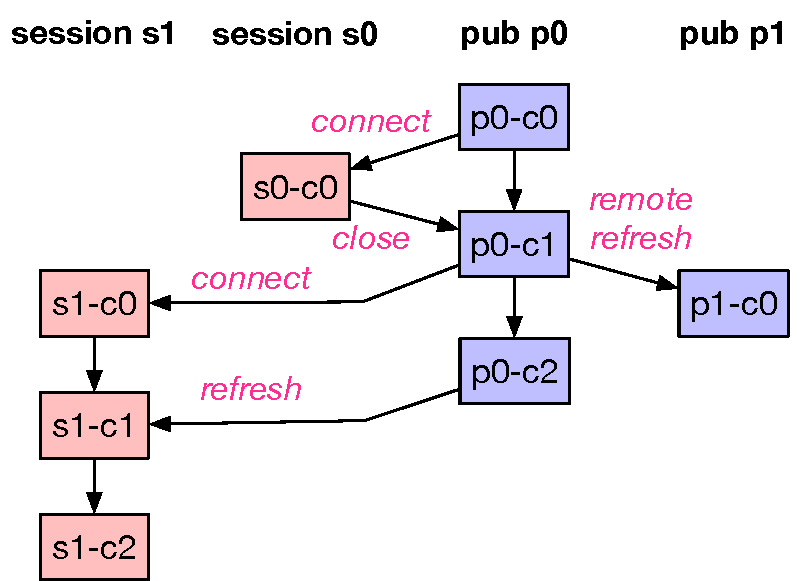
\includegraphics[scale=0.45]{figures/gc}
	\caption{Garbage collection. Here, the commits \texttt{p0-c0} and
		\texttt{s0-c0} may be deleted.}
	\label{fig:gc}
	\vspace{-0.7cm}
\end{wrapfigure}
For individual sessions, once the session is closed, the corresponding entry in
the tag store, and all the commits by that session may be deleted. In the
execution history in Figure~\ref{fig:gc}, the commit node |s0-c0| may be
deleted. The next question is when can commits on public branch be deleted. For
each ongoing session in a replica, we maintain the latest commit in the public
branch against which |refresh| was performed. The earliest of such commits in
the public branch and its descendants must be retained, since they are
necessary for the three-way merge. For example, in Figure~\ref{fig:gc}, session
|s1| refreshed against |p0-c2|, and |s1| is the only ongoing session. If |s1|
publishes, then |p0-c2| will be the LCA commit.

A similar reasoning is used for remote refreshes. When a commit in the public
branch of a replica has been merged into the public branches of all the other
replicas, then the ancestors of such commits will not be accessed and can be
deleted. In Figure~\ref{fig:gc}, assume that we only have two replicas. Since
|p0-c1| was merged by the public branch |p1|, |p0-c1| will be the LCA commit
for subsequent remote refreshes by |p1|. Given that |p0-c0| is neither
necessary for remote refreshes nor for ongoing sessions, |p0-c0| can be
deleted.
